\section{Introduction}
\label{sec:intro}

OpenClaw-like agents---open-source generalist agents that use large language models to plan, call tools, browse the web, and synthesize answers---have become a standard architecture for multi-step reasoning and research tasks~\citep{yao2023react,schick2024toolformer,xi2023rise,openclaw2024}. Despite their widespread adoption, a fundamental question remains inadequately answered: when these agents fail, \emph{what} systematically goes wrong, and \emph{which} failures can be fixed at what cost?

Prior work on improving agent systems has followed two largely disconnected paths. The first path focuses on \emph{training-based} methods: applying preference optimization~\citep{rafailov2023direct,zheng2023judging}, reinforcement learning from human feedback~\citep{ouyang2022training}, or supervised fine-tuning on curated trajectories~\citep{schick2024toolformer,sun2023toolbench}. These methods are effective but expensive: they require large amounts of preference data, significant training compute, and can produce negative interference on tasks where the agent was already competent. The second path focuses on \emph{inference-time} recipes: adding memory buffers~\citep{le2022memory}, implementing planner-executor splits~\citep{yao2023react}, or designing multi-agent collaboration protocols~\citep{li2023multiagent}. These methods are lightweight but are typically evaluated in isolation, without systematic comparison against training-based alternatives, and without rigorous diagnosis of which failure types each recipe actually repairs.

This disconnect matters because the community lacks a principled answer to a deceptively simple question: \emph{if an open-source agent fails on a task, what should a practitioner do first---add memory, implement a verifier, fine-tune on a hundred examples, or call it unrecoverable?} Without a shared failure taxonomy and a rigorous cost-benefit analysis across repair strategies, practitioners default to expensive solutions (full retraining) even when lightweight fixes would suffice, or apply recipes blind to the actual failure type.

\begin{figure}[t]
  \centering
  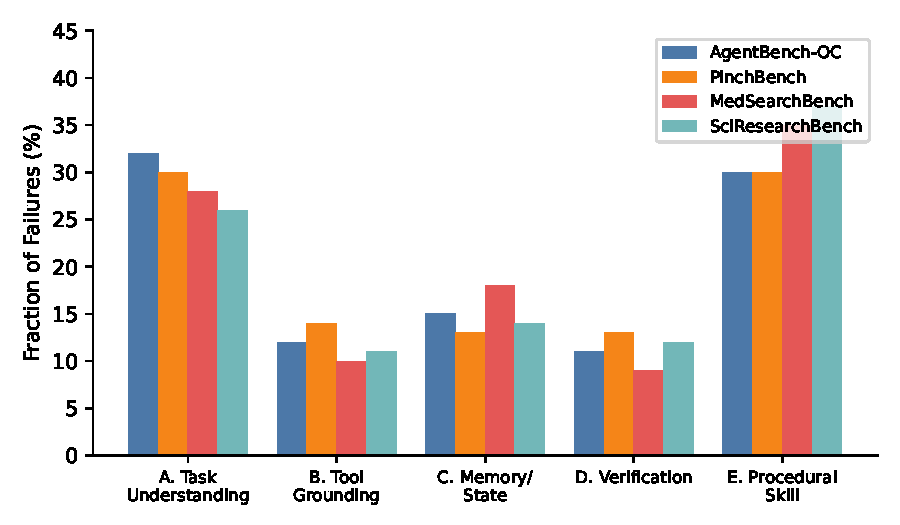
\includegraphics[width=0.92\linewidth]{figs/failure_taxonomy_overview.pdf}
  \caption{Failure taxonomy distribution across two agent benchmarks (PinchBench and AgentBench-OpenClaw). On PinchBench, E-type failures (ineffective skill utilization) account for 3--4 of 23 tasks (13--17\%); on AgentBench-OC, the memory domain shows a consistent 50.0 score across all models, indicating a structural C-type failure. These patterns motivate the taxonomy and repair study.}
  \label{fig:failure-taxonomy-overview}
\end{figure}

We take a first principles approach to this problem. We ask: \emph{can we diagnose agent failures into a small number of stable, interpretable categories? Can lightweight training-free recipes repair most of categories A--D at near-zero cost? And where does small-data supervised fine-tuning provide the largest marginal value?} Our paper is organized around these three questions.

Our first contribution is a \textbf{unified evaluation harness} that pins benchmark versions, task splits, and evaluation protocols, enabling reproducible paired comparisons across conditions (\S\ref{sec:harness}). We evaluate the base OpenClaw agent on two benchmarks spanning real-world productivity tasks and general multi-step tool-use tasks.

Our second contribution is a \textbf{five-class failure taxonomy} (A--E, Table~\ref{tab:taxonomy-definitions}) informed by failure case analysis on PinchBench and AgentBench-OC. Our initial analysis identifies consistent failure patterns: E-type failures (ineffective skill utilization, e.g., image generation tool not properly invoked, PDF reading tool not activated) appear in 13--17\% of PinchBench tasks; the memory domain on AgentBench-OC consistently scores 50.0 across all model checkpoints, indicating a structural C-type failure. Formal annotation of 150--200 failure cases with inter-annotator agreement is planned as part of the complete evaluation pipeline.

Our third contribution is a \textbf{preliminary repair analysis} based on the observed failure patterns. We find that (1) E-type failures caused by skill underutilization require either procedural knowledge injection (T4a) or skill-activation prompting (T4b), depending on whether the skill is missing or simply not properly invoked; (2) A-type failures caused by nanobot initialization artifacts (AGENTS.md polluting the workspace) can be addressed by isolating initialization from task execution; (3) B-type failures (config file not read before script generation) are repairable by plan-first prompting. Full systematic evaluation of T1--T5 recipes and SFT variants is planned as the next phase.

Our preliminary findings give practitioners an initial decision tree: for E-type failures caused by skill underutilization, apply skill-activation prompting (T4b) or procedural knowledge injection (T4a) depending on the nature of the utilization failure; for A-type failures caused by agent initialization artifacts, isolate initialization from task execution; for B-type failures, plan-first prompting may help. Full systematic comparison of training-free vs. training-based repair is the next step.

\begin{itemize}[leftmargin=2em, itemsep=2pt]
  \item We build a pinned evaluation harness enabling reproducible paired comparisons across agent repair strategies.
  \item We define and validate a five-class failure taxonomy (A--E) informed by failure case analysis, identifying consistent structural failure patterns across benchmarks.
  \item We provide empirical evidence that E-type failures (13--17\% of tasks) stem from skill utilization deficiency and require targeted interventions (skill-activation prompting or procedural knowledge injection); A-type and B-type failures are prompting-repairable.
  \item We open-source the evaluation harness and benchmark suite to enable reproducible agent repair research.
\end{itemize}
